\documentclass{article}
\usepackage{algorithmic}
\usepackage{algorithm}
\usepackage{graphicx}
\begin{document}
\title{B+ TREES}
\author{Ajay, Manjunath & Vaibhav }
\date{Thursday 18 March 2010 06:44:22 PM IST }
\maketitle

\section{DESCRIPTION}
\textbf{B+ Trees} \\
In computer science, a B+ tree (BplusTree) is a type of tree which represents sorted data in a way that allows for efficient insertion, retrieval and removal of records, each of which is identified by a key. It is a dynamic, multilevel index, with maximum and minimum bounds on the number of keys in each index segment (usually called a "block" or "node"). In a B+ tree, in contrast to a B-tree, all records are stored at the leaf level of the tree; only keys are stored in interior nodes.

The primary value of a B+ tree is in storing data for efficient retrieval in a block-oriented storage context — in particular, filesystems. This is primarily because unlike binary search trees, B+ trees have very high fanout (typically on the order of 100 or more), which reduces the number of I/O operations required to find an element in the tree.

Relational database management systems such as IBM DB2, Informix, Microsoft SQL Server, Oracle 8, Sybase ASI, PostgreSQL, Firebird and MySQL support this type of tree for table indices. Key-value database management systems such as Tokyo Cabinet and Tokyo Tyrant support this type of tree for data access. \\


\subsection{TIME AND SPACE COMPLEXITY}
For a b-order B+ tree with h levels of index:\\ 
    * The maximum number of records stored is nmax = bh\\
    * The minimum number of keys is nk = (b / 2)h − 1\\
    * The space required to store the tree is O(n)\\
    * Inserting a record requires O(logbn) operations in the worst case\\
    * Finding a record requires O(logbn) operations in the worst case\\
\pagebreak

\section {ALGORITHM}
\begin{algorithm}
\caption {ALGORITHM FOR INSERTION}
\begin {algorithmic}
\IF {$(ROOT \leftarrow null)$}
\STATE $ ROOT \leftarrow[key]  $
\ENDIF
\STATE $ INCREMENT COUNT and RETURN ROOT $
\STATE $ LEAF \leftarrow FIND LEAF(ROOT, key) $
\IF {$(LEAF HAS SPACE)$}
\STATE $ INSERT LEAF (LEAF, key) and RETURN ROOT $
\STATE $ RETURN SPLIT LEAF(ROOT, LEAF, key)$
\ENDIF 
\end{algorithmic}
\end{algorithm}

\pagebreak
\begin{algorithm}
\caption{ ALGORTIHM TO FIND LEAF }
\begin{algorithmic}
\STATE $ {NYPE find leaf(ROOT, key)} $
\IF {$(key exists in NODE)$}
\STATE $ ERROR MESSAGE \leftarrow No duplicates allowed and exit(0)$
\ENDIF
\IF {$(ROOT \leftarrow leaf)$}
\STATE $ RETURN ROOT $
\ENDIF
\STATE $FIND POSITION OF LINK$
\STATE $ FIND LEAF(ROOT \leftarrow LINK, key) $
\STATE ${NTYPE INSERT LEAF(LEAF, key)} $
\STATE $ FIND POSITION WHERE THE KEY HAS TO BE PLACED $
\STATE $ SHIFT ELEMENTS AHEAD TO MAKE ROOM FOR KEY $
\FOR {$(i\leftarrow LEAF\rightarrow COUNT to POSITION)$}
\STATE $ LEAF\rightarrow[i]=LEAF\rightarrow key[i-1] $
\ENDFOR
\STATE $LEAF\rightarrow KEY[POSITION]=key $
\STATE $INCREMENT COUNT $
\STATE $ RETURN COUNT $
\end{algorithmic}
\end{algorithm}

\pagebreak
\begin{algorithm}
\caption {AGORITHM TO SPLIT LEAF}
\begin{algorithmic}
\STATE $ {NTYPE SPLIT LEAF (ROOT, LEAF, key} $ 
\STATE $ COPY THE CONTENTS OF LEAF TO TEMP $
\FOR {$(i\leftarrow to LEAF\rightarrow COUNT)$}
\STATE $ TEMP[i]=LEAF\rightarrow key[i] $
\ENDFOR
\STATE $FIND POSITION WHERE KEY SHOULD BE PLACES $
\STATE $ SHIFT ELEMENTS TO MAKE ROOM FOR KEY $
\WHILE{$(position is less than order-1)$}
\STATE $temp[k]=temp[k-1] $
\STATE $DECREMENT k$
\ENDWHILE
\STATE $TEMP[POSITION]\leftarrow=key$
\STATE $ DETERMINE SPLIT LENGTH[(n/2)] $
\STATE $ PUT VALUES INTO LEAF $
\FOR {$(i=0 to length)$}
\STATE $LEAF\rightarrow key[i]=TEMP[i]$
\ENDFOR
\STATE $ PUT VALUES INTO NEW LEAF $
\FOR {$(i=length to order)$}
\STATE $NEW LEAF \rightarrow KEY[i]=TEMP[i]$
\STATE $INCREMENT j$
\ENDFOR
\STATE $NEW LEAF \rightarrow PARENT=LEAF\rightarrow PARENT $
\STATE $NEW LEAF \rightarrow SIBLING PTR = LEAF \rightarrow SIBLING PTR$
\STATE $ VAR=NEW LEAF\rightarrow key[0] $
\STATE $ RETURN INSERT PARENT (ROOT, LEAF, NEW LEAF, VAR) $
\end{algorithmic}
\end{algorithm}

\pagebreak
\begin{algorithm}
\caption{ALGORITHM TO INSERT PARENT}
\begin{algorithmic}
\STATE ${NTYPE INSERT PARENT(ROOT, LEAF1, LEAF2, VAR)} $
\STATE $ PARENT=LEAF1 \rightarrow PARENT $
\IF {$(PARENT=NULL)$}
\STATE $PARENT \rightarrow key[0]=VAR$
\STATE $ PARENT \rightarrow ptr[0]=LEAF1 $
\STATE $PARENT \rightarrow ptr[1]=LEAF2 $
\STATE $LEAF1\rightarrow =LEAF2\rightarrow PARENT $
\STATE $ RETURN PARENT $
\ENDIF
\STATE $ DETERMINE POSITION OF LINK FROM PARENT TO LEAF1 $
\STATE $ SHIFT POINTERS AND KEYS AHEAD TO MAKE SPACE $
\FOR {$(i=PARENT \rightarrow count to POSITION)$}
\STATE $ PARENT\rightarrow key[i]\rightarrow PARENT \rightarrow key[i-1] $
\STATE $ PARENT \rightarrow ptr[i+1]=PARENT \rightarrow ptrr[i] $
\ENDFOR
\STATE $ PARENT \rightarrow ptr[POSITION+1]=PARENT \rightarrow ptr[POSITION] $
\STATE $ PARENT \rightarrow key[POSITION]=VAR $
\STATE $ PARENT \rightarrow ptr[POSITION+1]=LEAF 2 $
\STATE $ RETURN ROOT $
\STATE $ RETURN SPLIT PARENT(ROOT, PARENT, LEAF2, POSITION, VAR) $
\end{algorithmic}
\end{algorithm}

\pagebreak

\begin{algorithm}
\caption{ALGORITHM FOR SPLIT PARENT}
\begin{algorithmic}
\STATE ${NTYPE SPLIT PARENT(ROOT, PARENT, LEAF2, POSITION, VAR)} $
\STATE $COPY POINTERS OF KEYS OF PARENT TO TEMP $
\FOR {$(i\leftarrow 0 to order-1)$}
\STATE $ TEMP(POINTER[i])=PARENT\rightarrow ptr[i] $
\STATE $ TEMP(POINTER[i])=PARENT\rightarrow key[i] $ 
\ENDFOR
\STATE $ TEMP(POINTER[order-1])=PARENT \rightarrow ptr[order-1] $
\STATE $ SHIFT POINTERS, KEYS AHEAD TO MAKE SPACE $
\FOR {$(i\leftarrow order-1 to POSITION)$}
\STATE $ TEMP(POINTERS[i+1]=TEMP(POINTERS[i]) $
\STATE $ TEMP(KEY[i])=TEMP(KEY[i-1]) $
\STATE $ TEMP(POINTER[POSITION+1])=LEAF2 $
\ENDFOR
\STATE $ TEMP(KEY[POSITION])=VAR $
\STATE $ ERASE PARENT $ 
\STATE $ COPY FIRST HALF OF POINTER, KEY TO PARENT $
\FOR {$(i \leftarrow to Plength)$}
\STATE $ PARENT \rightarrow ptr[i]=TEMP POINTER[i] $
\ENDFOR 
\STATE $ CPOY NEXT HALF OF THE POINTER, KEY TO NEW NODE $
\FOR {$(i= Plength to order-1)$}
\STATE $ NEW NODE \rightarrow ptr[j]=TEMP POINTER[i] $
\STATE $ INTERMEDIATE VALUE TO PASS $ 
\STATE $ Pvar = TEMP KEY [Klength] $
\STATE $ Connect child node of NEW NODE to NEW NODE $
\ENDFOR
\FOR {$(i=0 to NEW NODE \rightarrow COUNT)$}
\STATE $ NEW NODE \rightarrow ptr[i] \rightarrow =NEW NODE $
\ENDFOR
\STATE $ RETURN INSERT PARENT (ROOT, PARENT, NEW NODE, pvar ) $
\end  {algorithmic} 
\end {algorithm}
\pagebreak

\section{PROFILING}


\begin{table}[h]
\caption{B+ trees}
\centering


\begin{tabular}{|c|c|} 
\hline 
\hline 
no of elements  &  time taken in secs\\ 
\hline 

10000 & 0.020000\\ 
20000 &0.020000 \\
30000 & 0.040000 \\
40000 & 0.070000 \\
50000 & 0.100000 \\
\hline 

\end{tabular}
\end{table}
\begin{figure}
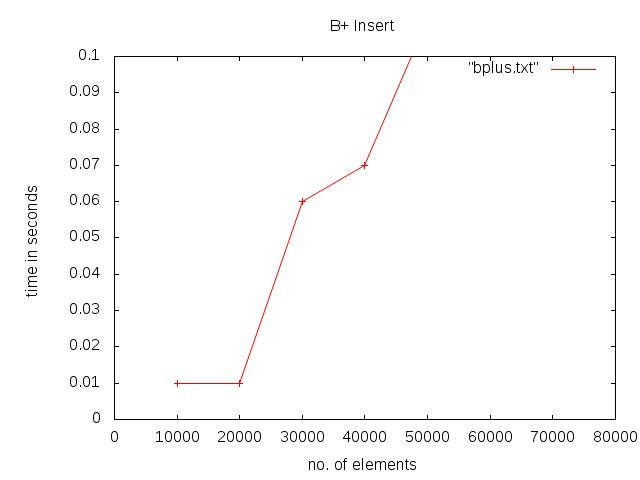
\includegraphics[height=3in,width=3in]{bplus.jpg}
\caption{Graph Plot Of B+ Trees}
\end{figure}

\pagebreak

\section{CONCLUSION}
 1. We successfully implemented B+ tree insertion which is used in various disk systems.\\
 2. Our code has three versions viz. 1.User-interface 2.Dotty-interface 3.Graph-plot using random function code.\\
 3. Looking at the above graph we can conclude that it takes very less time to insert/ access the data in the tree.\\
 4. To insert the first 10,000 -20,000 elements the graph value was a constant. After 20,000 + elements the growth was linear.\\
 5. This project helped us to re-inforce our programming skills.\\
 6. It also helped us to know the power of Linux(Ubuntu).

\end{document}
